\section{Background samples}

\subsection*{3 lepton background MonteCarlo}
To look for anomalies in the three lepton final state we need to train on background MonteCarlo samples with that specific final state. 
This means in a sense that we want the autoencoder to learn what is expected from the Standard model in terms of this final state. 
The 3 lepton background MonteCarlo contains the following channels:

\begin{enumerate}
    \item Wjets
    \item Triboson
    \item Higgs
    \item Zttjets
    \item Zmmjets
    \item Zeejets
    \item SingleTop
    \item TopOther
    \item ttbar
    \item Diboson2L
    \item Diboson3L
    \item Diboson4L
\end{enumerate}

Below are three examples of what some of the samples contains. The selected ones are likely Feynman diagrams for $t\bar{t}$, Higgs and Zeejets channels. 

\begin{figure}[h!]
    \centering
    \caption{Proton-proton collision showing the $t\bar{t}$ channel. Here the w bosons decay leptonically and one or more jets
    are misreconstructed as leptons by the detector. }

\begin{tikzpicture}
    \begin{feynman}
    
        \vertex at (0, 1.) (a2){\(g\)} ;
        \vertex at (0, -1.)  (a5){\(g\)} ;

        \vertex at (1.5, 1.) (c);
        \vertex at (3., 1.) (d);

        \vertex at (1.5, -1.) (e);
        \vertex at (3., -1.) (f);

        \vertex at (1.5, 1.) (g);
        \vertex at (1.5, -1.) (h);

        \vertex at (3, 1) (a1);
        \vertex at (4.5, 1.5) (a3);

        \vertex at (3, 1) (a6);
        \vertex at (4.5, 0.5) (a7);


        \vertex at (3, -1) (b1);
        \vertex at (4.5, -1.5) (b2);

        \vertex at (3, -1) (b3);
        \vertex at (4.5, -0.5) (b4);

       
        
    \diagram*{


        (a2) -- [gluon] (c) -- [anti fermion, edge label = {$\bar{t}$}] (d),
    
        (a5) -- [gluon] (e) -- [fermion, edge label = {$t$}] (f),

        (g) -- [fermion, edge label = {$t$}] (h),

        (a1) -- [boson, edge label ={$w^-$}] (a3),

        (a6) -- [anti fermion, edge label ={$\bar{b}$}] (a7),

        (b1) -- [boson, edge label ={$w^+$}] (b2),

        (b3) -- [anti fermion, edge label ={$b$}] (b4),
        
        ;
    };
    \end{feynman}
    \end{tikzpicture}
    \label{fig:ttbar_feynman}
    \end{figure}

    \begin{figure}[h!]
        \centering
        \caption{Proton-proton collision showing the Higgs channel. Here the Z bosons decay leptonically. }
    
    \begin{tikzpicture}
        \begin{feynman}
        
            \vertex at (0, 1.) (a2){\(g\)} ;
            \vertex at (0, -1.)  (a5){\(g\)} ;
    
            \vertex at (1.5, 1.) (c);
            \vertex at (3., 0) (d);
    
            \vertex at (1.5, -1.) (e);
            \vertex at (3., 0) (f);
    
            \vertex at (1.5, 1.) (g);
            \vertex at (1.5, -1.) (h);
    
            \vertex at (3, 0) (a1);
            \vertex at (4.5, 0) (a3);

            \vertex at (6, 1) (a6);
            \vertex at (6, -1) (a7);
    
           
            
        \diagram*{
    
    
            (a2) -- [gluon] (c) -- [anti fermion, edge label = {$\bar{t}$}] (d),
        
            (a5) -- [gluon] (e) -- [fermion, edge label = {$t$}] (f),
    
            (g) -- [fermion] (h),
    
            (a1) -- [dashed, edge label = {$H$}] (a3),

            (a3) -- [boson, edge label = {$Z$}] (a6),
            (a3) -- [boson, edge label = {$Z$}] (a7),


            
            ;
        };
        \end{feynman}
        \end{tikzpicture}
        \label{fig:higgs_feynman}
        \end{figure}
        
        \begin{figure}[h!]
            \centering
            \caption{Proton-proton collision showing the Zeejets channel. Here one of the Z bosons decay leptonically and the W boson
            decays hadronically. }
        
        \begin{tikzpicture}
            \begin{feynman}
                \vertex at (0, 1.) (a2){\(q\)} ;
                \vertex at (0, -1.)  (a5){\(\bar{q}^{'}\)} ;

                \vertex at (1.5, 1.) (c);

                \vertex at (1.5, -1.) (e);

                \vertex at (3, 1.) (b1);

                \vertex at (3, -1.) (b2);

                \vertex at (4.5, -0.5) (b4);

                \vertex at (4.5, -1.5) (b3);

                \vertex at (4.5, 0.5) (b5);

                \vertex at (4.5, 1.5) (b6);
        
                
               
                
            \diagram*{
        
        
                (a2) -- [fermion] (c),
            
                (a5) -- [anti fermion] (e),

                (c) -- [fermion] (e),

                (c) -- [boson, edge label={$Z$}] (b1),
                (e) -- [gluon, edge label={$g$}] (b2),

                (b2) -- [fermion, edge label={$b$}] (b4),
                (b2) -- [anti fermion, edge label={$\bar{b}$}] (b3),

                (b1) -- [fermion, edge label={$e^-$}] (b5),
                (b1) -- [anti fermion, edge label={$e^+$}] (b6),
        
                ;
            };
               
            \end{feynman}
            \end{tikzpicture}
            \label{fig:zeejets_feynman}
            \end{figure}

\subsection*{2 lepton background MonteCarlo}

\begin{enumerate}
    \item singletop 
    \item Diboson 
    \item Zeejets 
    \item Zmmjets 
    \item Zttjets 
    \item Wjets 
    \item ttbar
   
\end{enumerate}

 
\subsubsection*{Iterative training}
The two lepton dataset contains about 1.5 - 2 Terra bytes of data. This is too much to hold in memory at the same time, thus it had to be split into 
several smaller datasets, called megasets. Below is a figure visualizing the structure used. 

\begin{figure}[h!]
    \centering
    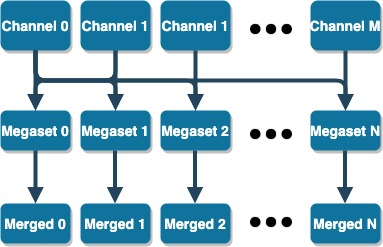
\includegraphics[width=0.6\linewidth]{Figures/2lep_config/megaset_struct.jpeg}
    \caption{Megaset structure for the 2lep dataset. This figure generalises to M channels, and N megasets. The more you increase the number of megasets, 
    the smaller each megaset will be in bytesize, but in order to keep the SM MC distribution, it is not recommended to make too small sets.  }
    \label{fig:2lep_struct}
\end{figure}




In figure \ref{fig:2lep_struct} we see a generalized dividing structure. In the case of this thesis, each channel was divided into 10 equal parts, 
and stored in their respective folder. When all channels were 
split, a merging was done combining all the channels in a given megaset to a separate dataset. The selection of events from each channel was done randomly, 
which is important, as we want to the best of our ability keep the distribution signature of the entire dataset in each megaset. If not, the model will 
be biased towards those datasets with the most events. Once each of the megasets where merged, the training could begin in an iterative fashion. Because
Tensorflow is statically compiled, you cannot call the fit function over and over again. Instead, the weights trained based on one megaset is stored and 
reloaded into a new model, thus the weights are still trained on the entire set, but in a batch like manner. 

\begin{lstlisting}[language=Python, style=pythonstyle, label={code:megabatch_training}]
for megaset in range(self.totmegasets):
    
    #* Load model 
    if SMALL:
        self.AE_model = nn_model.getModel()
    else:
        self.AE_model = nn_model.getModelBig()
    
    if megaset != 0:
        self.AE_model.load_weights('./checkpoints/Megabatch_checkpoint')
        
        
    #* Run Training
    with tf.device("/GPU:0"):

        tf.config.optimizer.set_jit("autoclustering")

        self.AE_model.fit(
            xtrain,
            xtrain,
            epochs=self.epochs,
            batch_size=self.b_size,
            validation_data=(xval, xval),
            sample_weight=x_train_weights,
        )
        
    
    self.AE_model.save_weights('./checkpoints/Megabatch_checkpoint')

\end{lstlisting}